\documentclass{article}
\usepackage{tikz}
\usetikzlibrary{chains}
\begin{document}

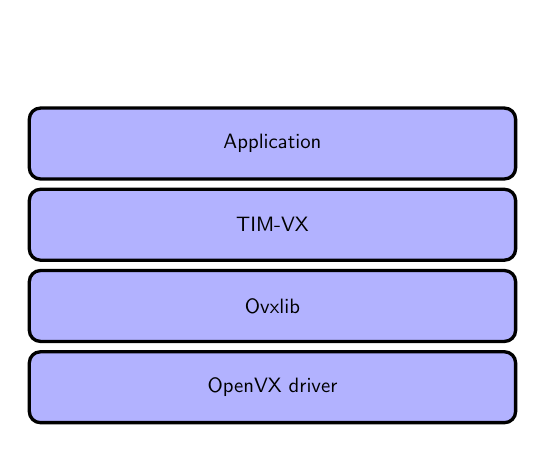
\begin{tikzpicture}[
	scale=0.75,
	start chain=1 going below, 
	node distance=1mm,
	desc/.style={
		scale=0.75,
		on chain=1,
		rectangle,
		rounded corners,
		draw=black, 
		very thick,
		text centered,
		text width=8cm,
		minimum height=12mm,
		fill=blue!30
		},
	it/.style={
		fill=blue!10
	},
	level/.style={
		scale=0.75,
		on chain=1,
		minimum height=12mm,
		text width=2cm,
		text centered
	},
	every node/.style={font=\sffamily}
]

% Levels
\node [level] (Level 3) {};
\node [level] (Level 2) {};
\node [level] (Level 1) {};
\node [level] (Level 0) {};

% Descriptions
\chainin (Level 3); % Start right of Level 5
% ICS levels
\node [desc] (App) {Application};
\node [desc] (TIMVX) {TIM-VX};
\node [desc] (Ovxlib) {Ovxlib};
\node [desc] (OpenVX) {OpenVX driver};

\end{tikzpicture}

\end{document}
